\documentclass[lang=cn,a4paper,11pt,openany,scheme=chinese,twoside]{elegantbook}

\let\arrowvert\relax
%\usepackage{unicode-math}

\let\arrowvert\relax

\usepackage{ctex}
\usepackage{xeCJK}
\usepackage{amsmath} % 建议
\usepackage{amssymb} % 可选,提供更多符号

\usepackage{ctex}
\let\openbox\relax

\usepackage{tikz}
\usetikzlibrary{decorations.pathreplacing,arrows.meta}

%调整页边距
\usepackage{geometry}
\geometry{top=2cm, bottom=2.25cm, outer=2cm, inner=2.5cm}


\usepackage{setspace}
\setstretch{1.3}

%设定行间距
\usepackage{calc}
\setlength{\lineskip}{\baselineskip-\ccwd}
\setlength{\lineskiplimit}{2.5pt}



%浮动图片
\usepackage{wrapfig}
%图标表格注记
\usepackage{caption}
%圆圈数字
\usepackage{pifont}
%表格换行
\usepackage{makecell}
%表格颜色
\usepackage[table]{xcolor}
\colorlet{rowcolcolor}{structurecolor!25!white}

%额外长度自适应箭标
\usepackage{extarrows}

%行间距加大
\newcommand{\wideline}{\setlength{\lineskip}{\baselineskip-\ccwd}\setlength{\lineskiplimit}{2.5pt}}
%蓝色加粗
\definecolor{titleblue}{HTML}{3498DB}
\newcommand{\bluebf}[1]{\textcolor{structurecolor}{\textbf{#1}}}


%向量
\usepackage[f]{esvect}

\renewcommand{\vector}[1]{\vv{#1}}
%平面
\newcommand{\plane}{\text{平面}\ }
%平行且等于
\newcommand{\paraleq}{%
    \mathrel{\text{%
        \tikz[baseline]
        \draw (.1em,0ex) -- (.9em,0ex)
        (.1em,-.425ex) -- (.9em,-.425ex)
        (.350em,.1ex) -- (.650em,1.5ex)
        (.550em,.1ex) -- (.850em,1.5ex);}}}

\newcommand{\mb}{\mathbb}
\newcommand{\z}{\text}
\renewcommand{\a}{\alpha}
\renewcommand{\b}{\beta}
\let\d\relax
\newcommand{\d}{\mathop{}\!\mathrm{d}}
\newcommand{\D}{\Delta}
\renewcommand{\l}{\lambda}
\newcommand{\m}{\mu}
\newcommand{\fl}{\fillin}
\newcommand{\pr}{\paren}
\newcommand{\p}{\uppi}
\renewcommand{\th}{\theta}
\newcommand{\lam}{\lambda}
\renewcommand{\leq}{\leqslant}
\renewcommand{\geq}{\geqslant}
\newcommand{\rttri}{\mathrm{Rt}\triangle}
\newcommand{\npar}{\par\noindent}
\DeclareSymbolFont{ugmL}{OMX}{mdugm}{m}{n}
\DeclareMathAccent{\wideparen}{\mathord}{ugmL}{"F3}
\newcommand{\sigmaalg}{\sigma-\text{代数}}
\newcommand{\setjot}[1][0]{\setlength{\jot}{#1 pt}}
\renewcommand{\cal}[1]{\mathcal{#1}}
\DeclareMathOperator{\st}{\text{s.t.}}
\DeclareMathOperator{\aew}{\text{a.e.}}


%填空题下划线
\newcommand{\fillin}[1][3.5]{%
  \nolinebreak % 不在此处断行
  \hspace{0.2em}%
  \rule[-0.5ex]{#1em}{0.5pt}% 轻微下沉模拟“下划线”效果
  \hspace{0.05em}
}

%调整环境内图片环绕
\usepackage{mwe}
\newcommand{\wrapfix}[1][-1]{\begin{wrapfigure}{r}{0.001\textwidth}%
    \vspace{#1 em}%
    \includegraphics[width=0.001\textwidth]{example-image}%
    \end{wrapfigure}}


%分式使用行间版
\everymath{\displaystyle}


\usepackage{myenvironment}


%elegantbook部分修改
\usepackage{elegantfix}

%强制右页开始
\makeatletter
\newcommand{\ForceRightPage}{%
  \clearpage
  \ifodd\value{page}\relax
    % 已经是奇数页,什么也不做
  \else
    \hbox{}\thispagestyle{empty}\newpage
  \fi
}
\makeatother

\raggedbottom


\begin{document}


\title{动力系统笔记}
\author{庞逸天}
\date{}
\maketitle
\setcounter{page}{1}

\frontmatter
\pagenumbering{roman}     % 目录等用罗马数字
\clearpage
\tableofcontents
\clearpage

\ForceRightPage
\mainmatter

\chapter{预备知识}

\section{概率测度空间}

\begin{definition}{$\sigma-$代数}
    设$X$是一个集合,$\mathcal{B}$是$X$的一些子集构成的集合类,若$\mathcal{B}$满足以下3个条件:
    \begin{enumerate}
        \item $X\in\mathcal{B}$
        \item $A\in\mathcal{B}\Rightarrow X\setminus A\in\mathcal{B}$
        \item $A_1,A_2,A_3,\cdots,A_n,\cdots\in\mathcal{B}\Rightarrow\bigcup_{i=1}^{\infty}{A_i\in\mathcal{B}}$
    \end{enumerate}
    则称$\mathcal{B}$是$X$的一个$\sigma-\text{代数}$
\end{definition}

除了上述定义中满足的三个条件之外,还可以证明$\sigma-\text{代数}$满足以下两个性质.

\begin{proposition}{$\sigma-\text{代数}$的基本性质}
    \begin{enumerate}
        \item $\varnothing\in\mathcal{B}$
        \item 设$A_i\in\mathcal{B}(i=1,2,\cdots,n)$,则$\bigcap_{i=1}^{\infty}{A_i}\in\mathcal{B}$   
    \end{enumerate}
\end{proposition}
\begin{proof}
    \begin{enumerate}
        \item 由条件1可知$X\in\mathcal{B}$,所以$X\setminus X\in\mathcal{B}$,即$\varnothing\in\mathcal{B}$.
        \item 由$A_i\in\mathcal{B}$知$A_i^c=X\setminus A_i \in\mathcal{B}$.所以$\bigcup_{i=1}^\infty{A_i^c}\in\mathcal{B}$
        $\Rightarrow X\setminus\left(\bigcup_{i=1}^\infty{A_i^c}\right)=\bigcap_{i=1}^\infty{A_i}\in\mathcal{B}$.
    \end{enumerate}
\end{proof}

因此,$\sigma-$代数是包含全集合$X$和空集$\varnothing$,且对取余,可数并和可数交运算均封闭的集类.我们也把$(X,\mathcal{B})$称为一个\bluebf{可测空间},把$(X,\mathcal{B})$中的元素叫做\bluebf{可测集}.下面我们引入可测空间上的测度.

\begin{definition}{概率测度}
    \wideline
    设$X$是一个集合,$\mathcal{B}$是$X$的一个$\sigma-\text{代数}$,函数:$m:\mathcal{B}\rightarrow[0,1]$.如果$m$满足以下2个条件:

    \begin{enumerate}
        \item $m(\varnothing)=0,m(X)=1$
        \item $\forall$两两不交集合$\{A_i\}_{i\in\mathbb{N}}(A_i\in\mathcal{B})$,$m\left(\bigcup_{i=1}^{\infty}{A_i}\right)=\sum_{i=1}^{\infty}{m(A_i)}$
    \end{enumerate}
    则称$m$为$(X,\mathcal{B})$上的一个概率测度,$(X,\mathcal{B},m)$是一个概率测度空间。
\end{definition}
特别地,如果在上面的定义中去掉$m(X)=1$的限制,则称$m$为\bluebf{有限测度},$(X,\mathcal{B},m)$为\bluebf{有限测度空间}.

\begin{instance}
    (1)取$X=[0,1]$,$\mathcal{B}=\{X\text{中的可测集}\}$,由可测集的性质可知$\mathcal{B}$是$X$的一个$\sigma$-代数.\par

    再令$m=m_{\mathrm{Leb}}:\mathcal{B}\rightarrow [0,1]$,其中$m_{\mathrm{Leb}}$为$\mathbb{R}$上的Lebesgue测度.\par
    由$m_{\mathrm{Leb}}(\varnothing)=0,m_{\mathrm{Leb}}([0,1])=1$以及Lebesgue测度的可列可加性可知$m_{\mathrm{Leb}}$是$(X,\mathcal{B})$的一个概率测度,$(X,\mathcal{B},m_{\mathrm{Leb}})$是一个概率测度空间.\par
    如果把$X$拓展到实数域$\mathbb{R}$,则$m_{\mathrm{Leb}}$就是一个有限测度,$(\mathbb{R},\mathcal{B},m_{\mathrm{Leb}})$是一个有限测度空间.\par
    (2)取$X=\{1,2,\cdots,n\}$,$\mathcal{B}=\{X\text{中的所有子集}\}$,同样可证$\mathcal{B}$是$X$的一个$\sigma$-代数.\par
    定义$m:{\setlength{\jot}{-0.5em}\begin{aligned}
        \mathcal{B}&\to [0,1]\\
        A&\mapsto \frac{|A|}{|X|}
    \end{aligned}}$,则有$m(\varnothing)=\frac{0}{n}=0$,$m(X)=\frac{n}{n}=1$.且若$A_1,A_2,\cdots,A_m$为$X$中两两不交子集,则$m\left(\bigcup_{i=1}^m{A_i}\right)=\frac{\left|\displaystyle\bigcup_{i=1}^m{A_i}\right|}{|X|}=\frac{\displaystyle\sum_{i=1}^m{|A_i|}}{|X|}=\sum_{i=1}^m{\frac{|A_i|}{|X|}}=\sum_{i=1}^m{m(A_i)}$.\par
    因此$m$是$(X,\mathcal{B})$上的概率测度,$(X,\mathcal{B},m)$是一个概率测度空间.\par
    如果我们把$X$看作一个样本空间,$m$实际上描述的就是古典概型中概率的定义.
\end{instance}

但很多时候,$\sigma-\text{代数}$上的测度不容易计算,因此我们需要引入\bluebf{半代数}与\bluebf{代数}的概念.
\begin{definition}{半代数}
    设$X$是一个集合,$\mathcal{S}$是由$X$的一些子集构成的集合类,如果$\mathcal{S}$满足以下3个条件:
    \begin{enumerate}
        \item $\varnothing\in\mathcal{S}$
        \item $A,B\in\mathcal{S}\Rightarrow A\cap B\in\mathcal{S}$
        \item $A\in\mathcal{S}\Rightarrow \exists\text{有限多个两两不交集合}E_i\in\mathcal{S}(i=1,2,\cdots,n)$,使得$X\setminus A=\bigcup_{i=1}^n{E_i}$
    \end{enumerate}
    称$\mathcal{S}$是$X$的一个半代数.
\end{definition}

\begin{instance}
    (1)取$X=[0,1]$,$\mathcal{S}=\{X\text{中所有区间}\}\cup\{\varnothing\}$.
    则$\mathcal{S}$是$X$的一个半代数.\par
    \begin{tikzpicture}[x=8cm,y=1cm,>=Latex,
  tick/.style={thick},
  braceA/.style={decorate,decoration={brace,amplitude=5pt},ultra thick,red!75},
  braceB/.style={decorate,decoration={brace,mirror,amplitude=4pt},ultra thick,blue!70},
  braceE/.style={decorate,decoration={brace,amplitude=5pt},ultra thick,orange!85!brown}
]

% ---------- 左图 ----------
% 数轴
\draw[tick] (-0.05,0)--(0.75,0) [->];
% 刻度与标签
\draw[tick] (0,0.08)--(0,-0.08) node[below=3pt] {$0$};
\draw[tick] (0.7,0.08)--(0.7,-0.08) node[below=3pt] {$1$};

% 区间端点(可根据需要调整)
\def\xA{0.15}  % A 的左端
\def\yA{0.00}
\def\xAmid{0.30} % A 与 B 的交叠开始
\def\xBend{0.50} % B 的右端

% A(红色,大括号)
\draw[braceA] (\xA,0.15) -- (0.4,0.15)
  node[midway,above=5pt,red!80] {$A$};
% B(蓝色,大括号)
\draw[braceB,blue] (0.3,-0.15) -- (0.5,-0.15)
  node[midway,below=5pt,blue] {$B$};

% 视觉上的端点竖线(与手绘一致,可选)
\draw[thick,red!75] (\xA,0.08)--(\xA,-0.08);
\draw[thick,red!75] (0.4,0.08)--(0.4,-0.08);
\draw[thick,blue!70] (0.3,0.08)--(0.3,-0.08);
\draw[thick,blue!70] (0.5,0.08)--(0.5,-0.08);

% 数学公式
\node at (0.35,-1.25) {$A,B\in\mathcal{S}\Rightarrow A\cap B\in\mathcal{S}$};

% ---------- 右图 ----------
\begin{scope}[xshift=6.5cm]
  % 数轴
  \draw[tick] (0.15,0)--(0.95,0) [->];
  % 刻度
  \draw[tick] (0.2,0.08)--(0.2,-0.08) node[below=3pt] {$0$};
  \draw[tick] (0.9,0.08)--(0.9,-0.08) node[below=3pt] {$1$};

  % 端点
  \def\xEoneL{0.2}  % E1 左
  \def\xEoneR{0.4}  % E1 右(也是 A 左)
  \def\xAtwoR{0.7}  % A 右(也是 E2 左)
  \def\xEtwoR{0.9}  % E2 右

  % E1 橙色
  \draw[braceE,orange!85!brown] (\xEoneL,0.15)--(\xEoneR,0.15)
     node[midway,above=6pt,orange!85!brown] {$E_1$};

  % A 红色
  \draw[braceA,red!75] (\xEoneR,0.15)--(\xAtwoR,0.15)
     node[midway,above=6pt,red!75] {$A$};

  % E2 橙色
  \draw[braceE,orange!85!brown] (\xAtwoR,0.15)--(\xEtwoR,0.15)
     node[midway,above=6pt,orange!85!brown] {$E_2$};

  % 端点竖线(可选)
  \foreach \p/\c in {\xEoneL/orange!85!brown,\xEoneR/red!75,\xAtwoR/orange!85!brown,\xEtwoR/orange!85!brown}{
    \draw[thick,\c] (\p,0.08)--(\p,-0.08);
  }

  \node at (0.55,-1.25) {$A\in\mathcal{S}\Rightarrow X\setminus A=E_1\cup E_2$};
\end{scope}
\end{tikzpicture}\par
(2)取$X=[0,1]^n$,$\mathcal{S}=\{X\text{中的所有矩体}\}\cup\{\varnothing\}$,则$\mathcal{S}$是$X$的一个半代数.
\end{instance}



\begin{definition}{代数}
    设$X$是一个集合,$\mathcal{A}$是$X$的一些子集构成的集合类,如果$\mathcal{A}$满足以下3个条件:
    \begin{enumerate}
        \item $\varnothing\in\mathcal{A}$
        \item $A,B\in\mathcal{A}\Rightarrow A\cap B\in\mathcal{A}$
        \item $A\in\mathcal{A}\Rightarrow A^c=X\setminus A\in\mathcal{A}$
    \end{enumerate}
    称$\mathcal{A}$是$X$的一个代数.
\end{definition}
结合第一个和第二个条件,还可以得到代数的以下性质:
\begin{proposition}{代数的性质}
    若$\mathcal{A}$是$X$的一个代数,则若$A_1,A_2,\cdots,A_n\in\mathcal{A}$,$\bigcup_{i=1}^n{A_i},\bigcap_{i=1}^n{A_i}\in\mathcal{A}$.
\end{proposition}
这说明代数是对取余、有限并和有限交封闭的集类,它和$\sigma-$代数的区别在于它不要求对可数并和可数交运算封闭.\par
从半代数的例子中可以看出,$[0,1]^n$内的矩体和空集构成半代数,相较于所有的可测集构成的$\sigma-\text{代数}$要简单许多,因此研究清楚半代数并将这些结论延申到$\sigma-$代数上也会比直接在$\sigma-$代数上做文章方便,为此,需要介绍\bluebf{最小代数}和\bluebf{延拓定理}.\par
\begin{definition}{最小代数}
    设$X$是一个集合,$\mathcal{S}$是$X$的一个半代数,定义\[\mathcal{A}(\mathcal{S})=\bigcap_{\substack{\mathcal{A}\supseteq\mathcal{S}\\\mathcal{A}\,\text{代数}}}{\mathcal{A}}\]
    则$\mathcal{A}(\mathcal{S})$是一个代数,称为包含$\mathcal{S}$的最小代数.
\end{definition}
下面我们证明$\mathcal{A}(\mathcal{S})$是一个代数.
\begin{proof}
    (1)$\varnothing\in\mathcal{A}(\mathcal{S})$\par
    (2)$A,B\in\mathcal{A}(\mathcal{S})\Rightarrow A,B\in\mathcal{A}(\mathcal{A}\subseteq\mathcal{S}) \Rightarrow A\cap B\in\mathcal{A}\Rightarrow A\cap B\in\mathcal{A}(\mathcal{S})$\par
    (3)$A\in\mathcal{A}(\mathcal{S})\Rightarrow A\in\mathcal{A}(\mathcal{A}\supseteq\mathcal{S}) \Rightarrow X\setminus A\in\mathcal{A}(\mathcal{A}\subseteq\mathcal{S})\Rightarrow X\setminus A\in\mathcal{A}(\mathcal{S})$
\end{proof}
\begin{remark}
    可以发现,在上述证明过程中并未使用到$\mathcal{S}$为半代数的性质,因此上述定义实际上并不依赖于$\mathcal{S}$为半代数.
\end{remark}
类似地,可以定义最小$\sigma-\text{代数}$的概念.
\begin{definition}{最小$\sigmaalg$}
    设$X$是一个集合,$\mathcal{S}$是$X$的一个半代数,定义\[\mathcal{B}(\mathcal{A})= \bigcap_{\substack{\mathcal{B}\supseteq\mathcal{A}\\\mathcal{B}\,\sigmaalg}}{\mathcal{B}}\]
    则$\mathcal{B}(\mathcal{A})$是一个$\sigmaalg$,称为包含$\mathcal{A}$的最小$\sigmaalg$.
\end{definition}
同样可以证明$\mathcal{B}(\mathcal{A})$为一个$\sigmaalg$.
\begin{proof}
    (1)$X\in\mathcal{B}(\mathcal{A})$\par
    (2)$A\in\mathcal{B}(\mathcal{A})\Rightarrow A\in\mathcal{B}(\mathcal{B}\supseteq\mathcal{A})\Rightarrow X\setminus A\in\mathcal{B}(\mathcal{B}\supseteq\mathcal{A})\Rightarrow X\setminus A\in\mathcal{B}(\mathcal{A})$\par
    (3)$A_1,A_2,\cdots,A_n,\cdots\in\mathcal{B}(\mathcal{A})\Rightarrow A_1,A_2,\cdots,A_n,\cdots\in\mathcal{B}(\mathcal{B}\supseteq\mathcal{A})\Rightarrow \bigcup_{i=1}^\infty{A_i}\in\mathcal{B}(\mathcal{B}\supseteq\mathcal{A}) \Rightarrow\bigcup_{i=1}^\infty{A_i}\in\mathcal{B}(\mathcal{A})$
\end{proof}
\begin{remark}
    同样地,上述定义也不依赖于$\mathcal{A}$是一个代数.
\end{remark}
除了上述的基本定义之外,我们发现可以用半代数的结构描述其最小代数.
\begin{theorem}
    设$X$是一个集合,$\mathcal{S}$是$X$的一个半代数,则$\mathcal{S}$生成的最小代数$\mathcal{A}(\mathcal{S})$的每个子集均能表示成$\mathcal{S}$中有限个互不相交元素的并,即:
    \[\mathcal{A}(\mathcal{S})=\left\{E=\bigcup_{i=1}^n{E_i}\bigg| E_i\in\mathcal{S},\,E_i\text{两两不交},\,n\in\mathbb{R} \right\}\]
\end{theorem}
\begin{proof}
    记$\mathcal{F}=\mathcal{A}(\mathcal{S})=\left\{E=\bigcup_{i=1}^n{E_i}\bigg| E_i\in\mathcal{S},\,E_i\text{两两不交},\,n\in\mathbb{R} \right\}$.\par
    \begin{enumerate}[label=(\arabic*)]
        \item $\mathcal{F}\supseteq\mathcal{S}$.\par
        令$n=1$即可.
        \item $\mathcal{F}$是$X$的一个代数
        \begin{enumerate}[label=(\roman*)]
            \item $\varnothing\in\mathcal{F}$
            \item 若$A,B\in\mathcal{F}$,则$A=E_1\cup\cdots\cup E_m(E_i\in\mathcal{S})$,$B=F_1\cup\cdots\cup F_n (F_i\in\mathcal{S})$.\par
            所以
            {\setlength{\jot}{-2pt}\begin{align*}
                A\cap B&=(E_1\cup\cdots\cup E_m)\cap(F_1\cup\cdots\cup F_n)\\
                &=(E_1\cap F_1)\cup(E_2\cap F_1)\cup\cdots\cup (E_m\cap F_1)\cup\cdots\\
                &=\bigcup_{\substack{1\leqslant i\leqslant m\\ 1\leqslant j\leqslant n}}(E_i\cap F_j)
            \end{align*}}
            其中$E_i\cap F_j\in\mathcal{S}$且它们两两不交.
            \item 若$A\in\mathcal{F}$,$A=E_1\cap E_2\cap\cdots\cap E_m(E_i\in\mathcal{S},\,\text{两两不交})$.\par
            则$X\setminus A = X\setminus (E_1\cup E_2\cup\cdots\cup E_m)=E_1^c\cup E_2^c\cup\cdots\cup E_m^c$.\par
            由半代数的性质可知,$E_i^c=\bigcup_{j=1}^{n_i}{F_{ij}}$,所以
            {\setlength{\jot}{-2pt}\setlength\belowdisplayskip{-10pt}\begin{align*}
                X\setminus A&=E_1^c\cup E_2^c\cup\cdots\cup E_m^c\\
                &=\bigcup_{j=1}^{n_1}{F_{1j}}\cap\bigcup_{j=1}^{n_2}{F_{2j}}\cap\cdots\cap\bigcup_{j=1}^{n_m}{F_{mj}} \\
                &=(F_{11}\cap F_{21}\cap F_{31}\cap\cdots\cap F_{m1})\cup\cdots \\
            \end{align*}}
            上式中的每一项都在$\mathcal{S}$中且两两不交.
        \end{enumerate}
    \end{enumerate}\par
    结合以上两点可知$\mathcal{F}\supseteq\mathcal{A}(\mathcal{S})$.
    \begin{enumerate}[label=(\arabic*)]
        \setcounter{enumi}{2}
        \item $F\subseteq\mathcal{A}(\mathcal{S})$\par
        $\forall \bigcup_{i=1}^n{E_i}\subset\mathcal{F},\, E_i\in\mathcal{S},\, E_i\text{两两不交},\,n\in\mathbb{N}$,$E_i\subseteq\mathcal{S}\subseteq\mathcal{A}(\mathcal{S})\Rightarrow \bigcup_{i=1}^n{E_i}\in\mathcal{A}(\mathcal{S})$.\par
        所以$\mathcal{A}(\mathcal{S})\supseteq\mathcal{F}$.
    \end{enumerate}\par
    综上可得$\mathcal{F}=\mathcal{A}(\mathcal{S})$.
\end{proof}
在建立起由半代数构造其最小代数的方法后,就可以把半代数上的某些函数延拓到其最小代数上,\bluebf{有限可加函数}是其中的一类.
\begin{definition}{有限可加(可列可加)函数}
    \wideline
    设$X$是一个集合,$\mathcal{S}$是一个半代数,$\tau:\mathcal{S}\to[0,1]$,如果
    \begin{enumerate}
        \item $\tau(\varnothing)=0$
        \item $\forall\bigcup_{i=1}^n{E_i}\in\mathcal{S},\, E_i\in\mathcal{S}(i=1,2,\cdots,n),\, E_i两两不交$,有$\tau\left(\bigcup_{i=1}^n{E_i}\right)=\sum_{i=1}^n{\tau(E_i)}$
    \end{enumerate}
    则称$\tau$是有限可加的.\par
    如果$n=\infty$,称$\tau$是可列可加的.
\end{definition}
显然,可列可加函数包含有限可加函数.\par
在代数$\mathcal{A}$和$\sigmaalg\mathcal{B}$上,也可以类似地定义有限可加函数和可列可加函数.例如概率测度空间$(X,\mathcal{B},m)$中的测度$m$是定义在$\sigmaalg\mathcal{B}$上的可列可加函数.\par
下面介绍半代数到其最小代数的延拓定理.\par
\begin{theorem}
    设$X$是一个集合,$\mathcal{S}$是一个半代数,$\tau:\mathcal{S}\to[0,1]$是一个有限可加(可列可加)函数,那么$\tau$可以唯一地延拓到$\mathcal{A}(\mathcal{S})$上的一个有限可加(可列可加)函数$\tau_1$.(即$\forall E\in\mathcal{S},\tau(E)=\tau_1(E)$)
\end{theorem}
\begin{proof}
    设$\tau:\mathcal{S}\to[0,1]$是一个有限可加函数,定义
    {\setlength{\jot}{-5pt}\begin{align*}
        \tau_1:\mathcal{A}(\mathcal{S})&\to[0,1]\\
        \bigcup_{i=1}^n{E_i}&\to\sum_{i=1}^n{\tau(E_i)}\,\,(E_i\in\mathcal{S},\,\text{两两不交})
    \end{align*}}
    \begin{itemize}
        \item 函数$\tau_1$是良定的.\par
        若$\bigcup_{i=1}^n{E_i}=\bigcup_{j=1}^m{F_j}\in\mathcal{A}(\mathcal{S})(E_i,F_j\in\mathcal{S})$,则
        {\setjot[-5]\begin{align*}
            \tau(E_i)&=\tau\left(E_i\cap\left(\bigcup_{j=1}^m{F_j}\right)\right)=\tau((E_i\cap F_1)\cup(E_i\cap F_2) \cup \cdots\cup(E_i\cap F_m) \\
            &=\tau(E_i\cap F_1)+\tau(E_i\cap F_2)+\cdots+\tau(E_i\cap F_m)=\sum_{j=1}^m\tau(E_i\cap F_j) \\
            \Rightarrow\sum_{i=1}^n\tau&(E_i)=\sum_{i=1}^n\sum_{j=1}^m{\tau(E_i\cap F_j)}
        \end{align*}}
        类似地,$\sum_{j=1}^m{\tau(F_j)}=\sum_{j=1}^m\sum_{i=1}^n{\tau(F_j\cap E_i)}$.\par
        所以$\sum_{i=1}^n{\tau(E_i)}=\sum_{j=1}^m{\tau(F_j)}$,$\tau_1$良定.
        \item 函数$\tau_1$有限可加.\par
        \begin{enumerate}[(1)]
            \item $\tau_1(\varnothing)=\tau(\varnothing)=0$
            \item 若$A_i\in\mathcal{A}(\mathcal{S})(i=1,2,\cdots,n)$两两不交.\par
            由代数的定义可知$A_i=\bigcup_{j=1}^{k_i}{E_{ij}},\,E_ij\in\mathcal{S},\,E_{ij}\text{两两不交},\, 1\leqslant j\leqslant k_i$.\par
            所以
            \vspace{-1em}
            {\setjot[-5]\begin{align*}
                \sum_{i=1}^n{\tau_1(A_i)}&=\tau_1(A_1)+\tau_1(A_2)+\cdots+\tau_1(A_n)\\
                &=\sum_{j=1}^{k_1}{\tau(E_{1j})}+\sum_{j=1}^{k_2}{\tau(E_{2j})}+\cdots+\sum_{j=1}^{k_n}{\tau(E_{nj})}\\
                &=\sum_{i=1}^n\sum_{j=1}^{k_i}{\tau(E_{ij})}=\tau\left(\bigcup_{i=1}^n\bigcup_{j=1}^{k_i}{E_{ij}}\right)\\
                &=\tau_1\left(\bigcup_{i=1}^n{A_i}\right)
            \end{align*}}
        \end{enumerate}
        \item 函数唯一\par
        如果$\tilde{\tau}$也满足条件,则$\tilde{\tau}=\tau_1$
    \end{itemize}
\end{proof}
类似地有代数$\mathcal{A}$到其最小$\sigmaalg\mathcal{B}(\mathcal{A})$的延拓定理.
\begin{theorem}
    设$X$是一个集合,$\mathcal{A}$是一个代数,$\tau:\mathcal{A}\to[0,1]$是$\mathcal{A}$上的一个可列可加函数,那么$\tau$可以唯一地延拓到$\mathcal{B}(\mathcal{A})$上的可列可加函数$m:\mathcal{B}(\mathcal{A})\to[0,1]$.(即$\forall A\in\mathcal{A},m(A)=\tau(A)$)
\end{theorem}
\begin{instance}
    设$X=[0,1]$,$\mathcal{S}=\{X\text{的所有子区间}\}$为一个半代数,$\mathcal{B}=\{X\text{中的可测集}\}$是一个$\sigmaalg$.\par
    在$\mathcal{S}$上定义函数$\tau:{\setjot[-7]\begin{aligned}
        \mathcal{S}&\to[0,1]\\
        I&\to|I|
    \end{aligned}}$,则$\tau$可延拓到$\mathcal{B}\left(\mathcal{A}(\mathcal{S})\right)$上的概率测度,其中$\mathcal{B}\left(\mathcal{A}(\mathcal{S})\right)$和$\mathcal{B}$只相差一个零测集.
\end{instance}

\section{单调类}
\vspace{-1em}
\begin{definition}{单调类}
    设$X$是一个集合,$\mathcal{C}$是$X$的一些子集构成的集合类,如果$\mathcal{C}$满足以下两个条件:
    \begin{enumerate}
        \item $\forall A_i\in\mathcal{C}(i\in\mathbb{N})$,$A_1\subseteq A_2\subseteq \cdots\subseteq A_n\subseteq\cdots\Rightarrow \bigcup_{i=1}^\infty{A_i}\in\mathcal{C}$
        \item $\forall A_i\in\mathcal{C}(i\in\mathbb{N})$,$A_1\supseteq A_2\supseteq\cdots\supseteq A_n\supseteq\cdots\Rightarrow\bigcap_{i=1}^\infty A_i\in\mathcal{C}$
    \end{enumerate}
    则称$\mathcal{C}$是$X$的一个单调类.
\end{definition}

单调类满足下述的一个基本性质.
\begin{proposition}{单调类的基本性质}
    如果$\mathcal{C}_i(i\in I)$是$X$的单调类,则$\bigcap_{i\in I}{\mathcal{C}_i}$是单调类.
\end{proposition}
\begin{proof}
    记$\mathcal{C}=\bigcap_{i\in I}{\mathcal{C}_i}$.若$A_1\subseteq A_2\subseteq\cdots \subseteq A_n\subseteq\cdots$,其中$A_i\in\mathcal{C}$.\par
    则$A_1\subseteq A_2\subseteq\cdots\subseteq A_n\subseteq\cdots$,其中$A_i\subseteq \mathcal{C}_k,k\in I$.\par
    $\Rightarrow \bigcup_{i=1}^\infty{A_i}\subseteq\mathcal{C}_k(k\in I)\Rightarrow \bigcup_{i=1}^\infty{A_i}\in\mathcal{C}$.\par
    对单调减的条件类似可证.
\end{proof}
该性质不论单调类是有限个还是无限个,是可数个还是不可数个,它们的交集都还是单调类.\par
对于任意一个集合$X$,它的所有子集构成的$X$的幂集$2^X$一定是包含$X$的一个单调类,因此任何集合都有包含它的单调类.因此,仿照半代数的最小代数、代数的最小$\sigmaalg$,我们可以定义一个集合生成的最小单调类.
\begin{definition}{最小单调类}
    设$\mathcal{S}$是$X$的一些子集构成的集合类,定义
    \[\mathcal{C}(\mathcal{S})=\bigcap_{\substack{\mathcal{C}\supseteq\mathcal{S}\\ \mathcal{C}\,\text{单调类}}}{\mathcal{C}}\]
    称为包含$\mathcal{S}$的最小单调类.
\end{definition}

下面一个定理介绍了一个代数生成的最小单调类和最小$\sigmaalg$之间的关系.
\begin{theorem}\label{thm:1.4}
    设$X$是一个集合,$\mathcal{A}$是$X$的一个代数,则$\mathcal{C}(\mathcal{A})=\mathcal{B}(\mathcal{A})$.
\end{theorem}
\begin{proof}
    由于$\mathcal{B}(\mathcal{A})$是一个$\sigmaalg$,所以$\mathcal{B}(\mathcal{A})$中任意子集的可数交与可数并包含于$\mathcal{B}(\mathcal{A})$,因此$\mathcal{B}(\mathcal{A})$是一个单调类,所以$\mathcal{B}(\mathcal{A})\supseteq\mathcal{C}(\mathcal{A})$.\par
    现证$\mathcal{C}(\mathcal{A})\supseteq\cal{B}(\cal{A})$,由于$\cal{C}(\cal{A})\supseteq\cal{A}$,所以只需证明$\cal{C}(\cal{A})$是一个$\sigmaalg$.
    \begin{itemize}
        \item 取补运算在$\mathcal{C}(\mathcal{A})$中封闭.\par
        定义$\mathcal{F}=\{E\in\mathcal{C}(\mathcal{A})|X\setminus E\in\mathcal{C}(\mathcal{A})\}$,现证$\mathcal{F}=\mathcal{C}(\mathcal{A})$.
        \begin{enumerate}[(\roman*)]
            \item 由定义可知$\mathcal{F}\subseteq\mathcal{C}(\mathcal{A})$.\par
            \item 由代数的定义可知$\forall A\in\mathcal{A}\subseteq\mathcal{C}(\mathcal{A}),X\setminus A\in\mathcal{A}\Rightarrow A\in\mathcal{F}(\forall A\in\mathcal{A}) \Rightarrow\mathcal{A}\subseteq\mathcal{F}$.
            \item $\mathcal{F}$是一个单调类.\par
            设$A_1\subseteq A_2\subseteq\cdots\subseteq A_n\subseteq\cdots (A_i\in \mathcal{F})$,则$A_i\in \mathcal{C}(\mathcal{A}),X\setminus A_i\in \mathcal{C}(\mathcal{A})$.\par
            $\xLongrightarrow{\text{单调类定义}}\bigcup_{i=1}^\infty{A_i} \subseteq \mathcal{C}(\mathcal{A}),\bigcap_{i=1}^\infty{(X\setminus A)} \in \mathcal{C}(\mathcal{A})$\par
            $\Rightarrow\bigcup_{i=1}^\infty{A_i} \subseteq \mathcal{C}(\mathcal{A}),X\setminus\left(\bigcup_{i=1}^\infty{A}\right) \in \mathcal{C}(\mathcal{A}) \Rightarrow \bigcup_{i=1}^\infty{A_i} \in \mathcal{F}$.\par
            对单调减的情形同理可证.因此,$\mathcal{F}$是单调类.
        \end{enumerate}
        由(ii)(iii)可得$F\supseteq\mathcal{C}(\mathcal{A})$.结合(i)得$\mathcal{F}= \mathcal{C}(\mathcal{A})$.
        \item 交运算在$\mathcal{C}(\mathcal{A})$中封闭.\par
        设$E\in \mathcal{C}(\mathcal{A})$,考虑$\mathcal{F}=\{A\in \mathcal{C}(\mathcal{A})|A\cap E\in \mathcal{C}(\mathcal{A})\}$,现证$\mathcal{F}= \mathcal{C}(\mathcal{A}$.
        \begin{enumerate}[(\roman*)]
            \item 由定义知$\mathcal{F}\supseteq \mathcal{A}$.
            \item $\mathcal{F}\supseteq\mathcal{A}.$($\forall B\in \mathcal{A},\forall F\in \mathcal{C}(\mathcal{A}),B\cap F\in\mathcal{C}(\mathcal{A})\Rightarrow B\in\mathcal{F}(\forall B\in \mathcal{A}) \Rightarrow \mathcal{A} \subseteq \mathcal{F}$)
            \item $\mathcal{F}$是一个单调类.\par
            设$A_1 \subseteq A_2 \subseteq \cdots \subseteq A_n \subseteq \cdots(A_i \in \mathcal{F})$,则$A_i \in \mathcal{C}(\mathcal{A}),A_i\cap E \in \mathcal{C}(\mathcal{A})$.\par
            $\xLongrightarrow{\text{单调类定义}}\bigcup_{i=1}^\infty{A_i} \in \mathcal{C}(\mathcal{A}),\left(\bigcup_{i=1}^\infty{A_i}\right)\cap E \in \mathcal{C}(\mathcal{A})\Rightarrow \bigcup_{i=1}^\infty{A_i} \in \mathcal{F}$.\par
            对单调减的情形同理可证,因此$\mathcal{F}$是单调类.
        \end{enumerate}
        由(ii)(iii)可得$F\supseteq\mathcal{C}(\mathcal{A})$.结合(i)得$\mathcal{F}= \mathcal{C}(\mathcal{A})$.
        \item $\mathcal{C}(\mathcal{A})$是一个$\sigmaalg$.\par
        \begin{enumerate}[(1)]
            \item $\varnothing\in\mathcal{C}(\mathcal{A})$.
            $\left(\varnothing\in\mathcal{A}\Rightarrow X=\varnothing^c \in \mathcal{A} \subseteq \mathcal{C}(\mathcal{A}) \Rightarrow \varnothing=X^c \in \mathcal{C}(\mathcal{A})\right)$.
            \item $A \in \mathcal{C}(\mathcal{A}) \Rightarrow A^c \in \mathcal{C}(\mathcal{A})$.
            \item $A_i \in \mathcal{C}(\mathcal{A})(i=1,2,\cdots) \Rightarrow \bigcup_{i=1}^\infty{A_i} \in \mathcal{C}(\mathcal{A})$.\par
            对于$A_1,A_2,\cdots,A_n$,$A_i^c \in \mathcal{C}(\mathcal{A}) \Rightarrow \bigcap_{i=1}^n{A_i^c} \in \mathcal{C}(\mathcal{A}) \Rightarrow \bigcup_{i=1}^n{A_i}=\left(\bigcap_{i=1}^n{A_i^c}\right)^c \in \mathcal{C}(\mathcal{A})$.\par
            $\left\{\bigcup_{i=1}^n{A_i}\right\}_{n=1}^\infty \in \mathcal{C}(\mathcal{A})$单调递增,所以$\bigcup_{i=1}^\infty{A_i} \in \mathcal{C}(\mathcal{A})$.
        \end{enumerate}
    \end{itemize}
\end{proof}
该定理指出要将代数$\mathcal{A}$扩张至其最小$\sigmaalg\mathcal{B}(\mathcal{A})$,只需要将$\mathcal{A}$中单调增集合序列的并集和单调减集合序列的交集包含进来即可.\par
之前在讨论最小代数和最小$\sigmaalg$时,已经给出了使用半代数中的元素构造其最小代数的方法.但对于代数生成的最小$\sigmaalg$中的元素,我们却一般无法详细描述,只能使用$\mathcal{A}$中的元素逼近$\mathcal{B}(\mathcal{A})$中的元素。下面我们可以借助$\mathcal{C}(\mathcal{A}) = \mathcal{B}(\mathcal{A})$来证明这种逼近关系.

\begin{theorem}
    设$(X,\mathcal{B},m)$为概率测度空间,$\mathcal{A}$是$X$的一个代数,$\mathcal{B} = \mathcal{B}(\mathcal{A})$,那么对于$\forall B \in \mathcal{B},\forall\varepsilon >0,\exists A \in \mathcal{A}$使得$m(A\triangle B)<\varepsilon$.
\end{theorem}
\begin{proof}
    设$\mathcal{F}=\{B\in\mathcal{B}|\forall \varepsilon>0, \exists A \in \mathcal{A} , m(A\triangle B)<\varepsilon\}$,现证$\mathcal{F}=\mathcal{B}=\mathcal{B}(\mathcal{A})$.由定义知$\mathcal{F}\subseteq\mathcal{B}$,故只需证明$\mathcal{F} \supseteq \mathcal{B}$\par
    \begin{enumerate}[(i)]
        \item $\mathcal{A}\subseteq\mathcal{F}$
        \item $\mathcal{F}$是一个单调类.\par
        设$B_1\subseteq B_2 \subseteq\cdots\subseteq B_n \subseteq\cdots(B_i \subseteq \mathcal{F},i \in \mathbb{N})$.\par
        由$\mathcal{F}$的定义可知$\forall\varepsilon>0, \exists A_i \in \mathcal{A}$,使得$m(A_i \triangle B_i)< \frac{\varepsilon}{2^i}$.\par
        由于$m\left(\bigcup_{i=1}^\infty{B_i}\right)\leqslant 1$,所以$\forall \varepsilon>0,\exists l \in \mathbb{N}$,使得$m\left( \bigcup_{i=l+1}^\infty{A_i} \right) < \varepsilon$,那么
        \begin{align*}
            m\left(\bigcup_{i=1}^l{A_i} \,\triangle\, \bigcup_{i=1}^\infty{B_i} \right) &= m\left(\left( \bigcup_{i=1}^l{A_i} \setminus \bigcup_{i=1}^\infty{B_i} \right) \cup \left( \bigcup_{i=1}^\infty{B_i} \setminus \bigcup_{i=1}^l{A_i} \right)\right) \\
            &= m\left( \bigcup_{i=1}^l{A_i} \setminus \bigcup_{i=1}^\infty{B_i} \right) + m\left( \bigcup_{i=1}^l{B_i} \setminus \bigcup_{i=1}^l{A_i} \right) + m\left( \bigcup_{i=l+1}^\infty{B_i} \setminus \bigcup_{i=1}^l{A_i} \right) \\
            &\leqslant m\left( \bigcup_{i=1}^l{A_i} \setminus \bigcup_{i=1}^l{B_i} \right) + m\left( \bigcup_{i=1}^l{B_i} \setminus \bigcup_{i=1}^l{A_i} \right) + m\left( \bigcup_{i=l+1}^\infty{B_i} \right) \\
            &\leqslant\sum_{i=1}^l{m(A_i \,\triangle\, B_i)} + m\left( \bigcup_{i=l+1}^\infty{B_i} \right) \\
            &\leqslant \varepsilon + \varepsilon = 2\varepsilon
        \end{align*}
        $\Rightarrow \bigcup_{i=1}^\infty{B_i} \in \mathcal{F}$.\par
        对于单调减的情形同理可证.
    \end{enumerate}\par
    进而可知$\mathcal{F} \supseteq \mathcal{C}(\mathcal{A}) \xLongrightarrow{\text{定理}\ref{thm:1.4}}\mathcal{F}\supseteq \mathcal{B}({A}) = \mathcal{B}$.\par
    综上得$\mathcal{F}=\mathcal{B}(\mathcal{A})$.
\end{proof}
\begin{remark}
    上述证明过程中除了最后一步实际上并未使用单调集的性质,因此也可以脱离单调集,仅使用$\sigmaalg$相关概念证明$\mathcal{F} \supseteq \mathcal{B}(\mathcal{A})$.\par
    \begin{proof}
        (1)$\forall B_i \in \mathcal{F} \Rightarrow \bigcup_{i=1}^\infty{B_i} \in \mathcal{F}$.\par
        (2)$B \in \mathcal{F} \Rightarrow \forall \varepsilon>0,\exists A \in \mathcal{A}$,使得$m(A \triangle B)=m(A \setminus B)+m(B \setminus A)=m(B \setminus A^c)+m(A\setminus B^c)=m(A^c \triangle B^c)<\varepsilon \Rightarrow B^c \in \mathcal{F}$.\par
        结合(1)(2)两点知$\mathcal{F}$为$\sigmaalg$,所以$\mathcal{F} \supseteq \mathcal{B}(\mathcal{A})$
    \end{proof}
\end{remark}

\section{积概率空间}

假设$(X_i,\mathcal{B}_i,m_i)$为一列概率测度空间$-\infty<i<+\infty,i\in\mathbb{Z}$,我们定义集合
\[X=\prod_{i=-\infty}^{+\infty}{X_i}=\left\{(\cdots,x_{-1},x_0,x_1,\cdots)|x_i \in X_i\right\}\]
在这个集合上可以定义其半代数.
\begin{definition}{可测矩形}
    $\mathcal{S}=\left\{ \prod_{i=1}^{m-1}{X_i} \times A_m \times A_{m+1} \times \cdots \times A_{n-1} \times A_n \times \prod_{i=n+1}^{+\infty}{X_i} : A_k \in \mathcal{B}_k, m \leqslant k \leqslant n,\;m,n \in \mathbb{Z}\right\}$,称其为可测矩形,它是$X=\prod_{i=-\infty}^{+\infty}{X_i}$的半代数.
\end{definition}

利用该半代数和前面提到的利用半代数生成代数、用代数生成$\sigmaalg$的方法,我们可以定义$X$上的$\sigmaalg$.
\begin{definition}{积$\sigmaalg$}
        定义$\mathcal{B}= \mathcal{B}(\mathcal{A}(\mathcal{S}))$,称为积$\sigmaalg$,为$X=\prod_{i=-\infty}^{+\infty}{X_i}$上的$\sigmaalg$.
\end{definition}
类似地,我们可以通过在可测矩形上定义$\tau$函数并将其延拓到$\mathcal{B}(\mathcal{A}(\mathcal{S})))$来得到$(X,\mathcal{B})$上的概率测度.
\begin{definition}{积测度}
    在$\mathcal{S}$上定义
    \begin{align*}
        \tau:\mathcal{S}&\to[0,1] \\
        \prod_{i=1}^{m-1}{X_i} \times A_m \times \cdots \times A_n \times \prod_{i=n+1}^{+\infty}{X_i} &\mapsto m_m(A_m) \times \cdots \times m_n(A_n)
    \end{align*}
    将$\tau$唯一地延拓到$\mathcal{B}=\mathcal{B}(\mathcal{A}(\mathcal{S}))$,可以得到$\mathcal{B}$上的概率测度,记为$m$,叫做积测度.
\end{definition}
由此,我们就得到了$X$上的$\sigmaalg$和相应的测度,它们构成了一个概率测度空间.
\begin{definition}{积概率空间}
    上述的$(X,\mathcal{B},m)$称为$(X_i,\mathcal{B}_i,m_i)$的积概率空间,记作$\prod_{i=-\infty}^{+\infty}{(X_i,\mathcal{B}_i,m_i})$
\end{definition}
类似地,可以相应定义$\prod_{i=0}^\infty{X_i}$和$\prod_{i=-\infty}^0{X_i}$.\par
在本课程中,通常遇到的积概率空间是由完全相同的概率测度空间构成的,其中每一个概率测度空间中的测度均为离散测度.\par
\begin{instance}
    $X_i={1,2,\cdots,n}\qquad \mathcal{B}_i=\{ X_i\text{的所有子集}\}$\par
    $\setjot\begin{aligned}
        m_i:B_i&\to[0,1] \\
        A&\mapsto\frac{|A|}{n}
    \end{aligned} \quad \Rightarrow(X_i,\mathcal{B}_i,m_i)$\par
    $X=\prod_{i=-\infty}^\infty{X_i}$.
\end{instance}


\section{积分与测度相关概念}

\begin{definition}{Borel $\sigmaalg$}
    设$X=\mathbb{R}$,包含所有开集的最小$\sigmaalg$称为Borel $\sigmaalg$$\mathcal{B}(\mathbb{R})$.
\end{definition}

借助Borel $\sigmaalg$,可以定义$(X,\mathcal{B},m)$上的可测函数,这里给出其等价定义.
\begin{definition}{可测函数}
    设$(X,\mathcal{B},m)$概率测度空间,对于函数$f:X\to\mathbb{R}$,如果$\forall c \in \mathbb{R}$,$f^{-1}\left((-\infty,c)\right) \in \mathbb{R}$,则称$f$是一个可测函数.
\end{definition}

下面仿照实变函数中Lebesgue积分的定义方式定义从简单函数到一般可测函数在概率测度空间上的积分.

\begin{definition}{积分}
    \wideline
    \begin{enumerate}
        \item 若$\varphi(x) = \sum_{i=1}^n{c_i \chi_{A_i}(x)}$为一个简单函数,$\int_X{\varphi(x)}\d m = \sum_{i=1}^n{c_i m(A_i)}$.
        \item 若$f\geqslant 0$可测函数,有简单函数逼近$\varphi_n(x) \nearrow f(x)$,则$\int_X{f}\d m=\sup_{n\to\infty}\int_X{\varphi_n(x)\d m}$.
        \item 若$f$一般可测函数,$f=f^++f^-$,$f^+=\max\{f,0\}, f^-=\max\{-f,0\}$,则$\int_X{f}\d m = \int_X{f^+}\d m - \int_X{f^-}\d m$.
    \end{enumerate}
\end{definition}

在概率测度空间中定义的上述积分依旧满足以下定理和引理.

\begin{theorem}{Levi定理 MCT}
    设$\{f_n\}_{i=1}^\infty$为$(X,\mathcal{B},m)$上的非负可积函数列.如果$f_n$关于$n$单调递增且$\left\{ \int_X{f_n}\d m \right\}$是有界数列,则极限$\lim_{n\to\infty}{f_n} = f$存在a.e.且可积,并满足
    \[\lim_{n\to\infty}{\int_X{f_n}\d m}=\int_{X}{f}\d m.\]
\end{theorem}
\begin{remark}
    在上述定理中,如果可知函数列极限几乎处处存在,则不需要函数列积分有界的条件.
\end{remark}

\begin{lemma}{Fatou引理}
    设$\{f_n\}_{i=1}^\infty$为$(X,\mathcal{B},m)$上的非负可测函数列.
    \begin{enumerate}[(i)]
        \item 如果存在可积函数$g$,使$f_n \geqslant g$对每一个$n=1,2,3,\cdots$成立,且
        \[ \liminf_{n\to\infty}{\int{f_n}}\d m <\infty, \]
        则$\liminf{f_n}$是可积的,且有
        \[\int{\liminf_{n\to\infty}{f_n}\d m} \leqslant \liminf_{n\to\infty}{\int{f_n}\d m}. \]
        \item 如果存在可积函数$g$,使$f_n \leqslant g$对每一个$n=1,2,3,\cdots$成立,且
        \[ \limsup_{n\to\infty}{\int{f_n}}\d m > -\infty, \]
        则$\limsup{f_n}$是可积的,且有
        \[\int{\limsup_{n\to\infty}{f_n}\d m} \geqslant \limsup_{n\to\infty}{\int{f_n}\d m}. \]
    \end{enumerate}
\end{lemma}

\begin{theorem}{Lebesgue控制收敛定理 LDCT}
    设$f_n:X\to\mathbb{R}$为$(X,\mathcal{B},m)$上的可测函数列且被一个可积函数$g:X\to\mathbb{R}$控制:$|f_n| \leqslant g,\,$a.e.,进一步设$\lim_{n\to\infty}{f_n} = f,\,$a.e. ,则$f$可积,且满足
    \[\lim_{n\to\infty}{\int{f_n}\d m} = \int{f}\d m. \]
\end{theorem}

下面的定义描述了同一空间上的两个概率测度之间的关联.

\begin{definition}{绝对连续}
    设$X$是一个集合,$\mathcal{B}$是$X$的一个$\sigmaalg$,$\mu,m$是$(X,\mathcal{B})$的概率测度.\par
    如果$\forall B \in \mathcal{B}$,$m(B)=0 \Rightarrow \mu(B)=0$,称$\mu$绝对连续于$m$,记为$\mu \ll m$.\par
    如果$\mu \ll m $且$m \ll \mu$,称$\mu$和$m$等价.
\end{definition}

除了上述的定义之外,我们也可以利用下述定理使用函数刻画何时$\mu \ll m$.

\begin{theorem}{Radon-Nikodym 定理}
    \wideline
    设$m$和$\mu$为可测空间$(X,\mathcal{B})$的两个概率测度,则$\mu \ll m$的充要条件是存在
    \[f \in L_1(m),\quad f \geqslant 0,\quad \int{f}\d m =1, \]
    使得对任意$C\in\mathcal{B}$,有$\mu(C) = \int_C{f}\d m$.\par
    此时的函数$f$是几乎处处唯一的.(如果$g$也满足这些性质,则$f=g\;$a.e. $x\in X$)
\end{theorem}

\begin{remark}
    上面定理中的函数$f$叫做$\mu$关于$m$的Radon-Nikodym 导数,记作$f=\frac{\d\mu}{\d m}$
\end{remark}

最后介绍Lebesgue覆盖引理和Lebesgue数的概念.
\begin{lemma}{Lebesgue 覆盖引理}
    设$(X,d)$是一个紧致度量空间,$\alpha$是$X$的一个开覆盖,那么$\exists \delta>0$,使得对于任意直径小于$\delta$的集合$B$,可以找到$U\in \alpha$,使得$B \subseteq U$,$\delta$称为此开覆盖的Lebesgue数.
\end{lemma}
\begin{proof}
    使用反证法,若$\forall n \in \mathbb{N},\delta=\frac{1}{n},\exists B_n \subset X,\operatorname{diam}B_n < \delta_n$,$B_n$不包含在$\alpha$的任何一个开集中.\par
    任取$x_n \in B_n$,$\{x_n\}_{n\in\mathbb{N}}$,由$(X,d)$为紧致度量空间,存在收敛子列$\{x_{n_k}\}_{k \in \mathbb{N}},x_{n_k}\to x_0 \in X$.\par
    由于$\alpha$是$X$的一个开覆盖,所以$\exists U_o\in\alpha$,使得$x_0\in U_0$.\par
    $\xLongrightarrow{U_0\textbf{为开集}} \exists\varepsilon>0,\,B(x_0,\varepsilon) \subseteq U_0$.\par
    当$k$充分大时,$B_{n_k}\subseteq B(x_0,\varepsilon) \subseteq U_0$.矛盾!
\end{proof}



\chapter{遍历理论}

\section{一个问题}

在正式介绍遍历理论之前,首先看一个利用遍历理论解决概率论问题的例子,以此引入我们将在后续学习的概念.问题是:
\begin{problem}
    考虑数列$x_n=2^{n-1}$,$a_n$表示$x_n$的第一位数字,
    则对$\forall k\in\{1,2,\cdots,9\}$,计算$P(a_n=k) =$?
\end{problem}
\begin{wrapfigure}{l}{0.15\textwidth}
    \vspace{-1.5em}
    \centering
    \renewcommand{\arraystretch}{1.1}
    \setlength{\tabcolsep}{10pt}
    \begin{tabular}{|c|c|c|}
        \hline
        $n$ & $x_n$ & $a_n$ \\
        \hline
        0 & 1 & 1 \\
        \hline
        1 & 2 & 2 \\
        \hline
        2 & 4 & 4 \\
        \hline
        3 & 9 & 9 \\
        \hline
        4 & 16 & 1 \\
        \hline
        5 & 32 & 3 \\
        \hline
    \end{tabular}
    \vspace{-12em}
\end{wrapfigure}\par
\vspace{0.5em}
首先对该问题进行化简,将其解释为可以处理的数学问题.\par
$\begin{aligned}
    x_n=2^n,a_n=x_n\text{的首一数字} &\Leftrightarrow \exists m\in\mathbb{N},\; \text{使得}a_n \cdot 10^m \leqslant 2^n \leqslant (a_m+1) \cdot 10^m \\
    &\xLongleftrightarrow{\text{取对数}}\log{a_m}+m \leqslant n\log{2} \leqslant \log{a_m+1} +m \\
    &\xLongleftrightarrow{\text{取小数部分}} \log{a_m} \leqslant \{n\log{2}\} \leqslant \log{(a_m+1)} \\
    &\Longleftrightarrow \{n\log{2}\} \in [\log{a_m},\log{(a_m+1)}]
\end{aligned}$\par
\vspace{2em}\par\noindent
\begin{itemize*}
    \item $P(a_n=k)=\lim_{N\to\infty}{\frac{\big|\{0 \leqslant n \leqslant N-1|a_n=k\}\big|}{|N|}}=\lim_{N\to\infty}{\frac{1}{N} \left( \sum_{n=0}^{N-1}{\chi_{I_k}\big(\{n\log{2}\}\big)}\right)},\;I_k \in [\log{k},\log{(k+1)}]$\par
\end{itemize*}

为了求出上述概率,我们需要引入均匀分布的概念.\par

\begin{definition}{均匀分布}
    设$\{x_n\}_{n\in\mathbb{N}} \subseteq [0,1]$,如果对于任意区间$I \subseteq [0,1]$,$\{x_n\}$落入区间$I$的概率等于$|I|$,即
    \[\lim_{n\to\infty}{\frac{\Big|\big\{1\leqslant n \leqslant N|x_n \in I\big\}\Big|}{N}} = |I|\]
    那么称$\{x_n\}_{n\in\mathbb{N}}$在$[0,1]$中均匀分布.
\end{definition}

下面还有均匀分布的等价刻画.
\begin{proposition}{均匀分布的等价刻画}
    $\{x_n\}_{n\in\mathbb{N}}$在$[0,1]$中均匀分布$\Longleftrightarrow\; \forall\, f\in C([0,1]), f(0)=f(1), \frac{1}{N}\sum_{n=1}^N{f(x_n)}\to \int_{0}^{1}{f(x)}\d x.$
\end{proposition}
\begin{proof}
    \begin{itemize}
        \item[“$\Rightarrow$”] 由均匀分布的定义可知,$\forall\, I \subseteq [0,1]$,$\frac{1}{N}\sum_{n=1}^N{\chi_{I}(x_n)} \to |I| = \int_0^1{\chi_{I}(x)}\d x$.\par
        则对简单函数$\varphi(x)=\sum_{i=1}^n{c_1\chi_{I_1}(x)}$,$\frac{1}{N}\sum_{n=1}^N{\varphi(x_n)}\to \int_{0}^{1}{\varphi(x)}\d x$.\par
        利用简单函数逼近一般可测函数$f(x)$, \par
        即$\forall\, \varepsilon>0,\exists\, \varphi(x)=\sum_{i=1}^n{c_i\chi_{I_i}(x)}$,s.t. $|\varphi(x)-f(x)| < \varepsilon(\forall\, x\in [0,1])$.\par
        故$\left\lvert \frac{1}{N}\sum_{n=1}^N{f(x_n)} - \frac{1}{N}\sum_{n=1}^N{\varphi(x_n)} \right\rvert \leqslant \frac{1}{N}\sum_{n=1}^N{\left\lvert f(x_n)-\varphi(x_n) \right\rvert} < \varepsilon$.\par
        $\Rightarrow \frac{1}{N}\sum_{n=1}^N{\varphi(x_n)} - \varepsilon \leq \frac{1}{N}\sum_{n=1}^N{f(x_n)} \leq \frac{1}{N}\sum_{n=1}^N{\varphi(x_n)} + \varepsilon$.\par
        令$n\to\infty$,取上下极限,其中下面两个不等号成立的原因是积分的绝对值不等式
        \begin{alignat*}{2}
            \int_0^1{\varphi(x)}\d x - \varepsilon &\leq \varliminf_{n\to\infty}{\frac{1}{N}\sum_{n=1}^N{f(x_n)}} \leq \varlimsup_{n\to\infty}{\frac{1}{N}\sum_{n=1}^N{f(x_n)}} &&\leq \int_0^1{\varphi(x)}\d x + \varepsilon  \\
            \int_0^1{f(x)}\d x - 2\varepsilon &\leq &&\leq \int_0^1{f(x)}\d x + 2\varepsilon
        \end{alignat*}
        令$\varepsilon\to 0 \Rightarrow \frac{1}{N}\sum_{n=1}^N{f(x_n)}\to \int_{0}^{1}{f(x)}\d x$.\par
    \end{itemize}
    \begin{minipage}[t]{0.8\textwidth}
    \begin{itemize}
        \item[“$\Leftarrow$"] $\forall\, I \subseteq [0,1]$,构造连续函数列$\{\varphi_n(x)\}_{n\in\mathbb{N}}$和$\{\psi_n(x)\}_{n\in\mathbb{N}}$,使
        \begin{enumerate}[(1)]
            \item $\varphi_n(x) \leq \chi_{I}(x) \leq \psi_n(x)$
            \item $\int_0^1{\varphi_n(x)}\d x \to \int_0^1{\chi_{I}(x)}\d x.$\par
            $\int_0^1{\psi_n(x)}\d x \to \int_0^1{\chi_{I}(x)}\d x.$\par
        \end{enumerate}
        $\Rightarrow \frac{1}{N}\sum_{n=1}^N{\varphi_n(x_n)} \leq \frac{1}{N}\sum_{n=1}^N{\chi_{I}(x_n)} \leq \frac{1}{N}\sum_{n=1}^N{\psi_n(x_n)}$.\par
        $\xLongrightarrow{n\to\infty}\int_0^1{\varphi_n(x)}\d x \leq \varliminf_{n\to\infty}{\sum_{n=1}^N{\chi_{I}(x_n)}} \leq \varlimsup_{n\to\infty}{\sum_{n=1}^N{\chi_{I}(x_n)}} \leq \int_0^1{\psi_n(x)}\d x$.\par
        $\Rightarrow \lim_{n\to\infty}{\sum_{k=1}^N{\chi_{I}(x_k)}} = \int_0^1{\chi_{I}(x)}\d x$.\par
    \end{itemize}
    \end{minipage}
    \begin{minipage}[t]{0.225\textwidth}
        \vspace{0 em}
        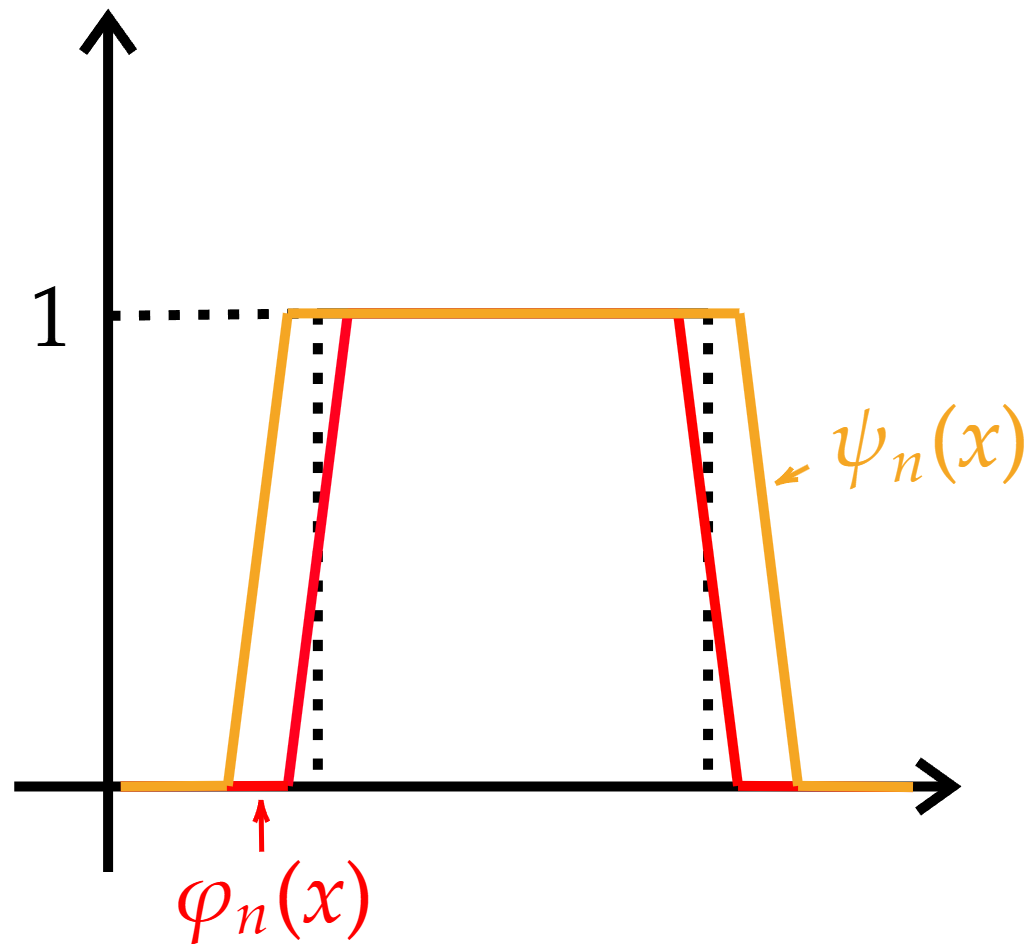
\includegraphics[width=1\textwidth]{fig/2.1.png}
    \end{minipage}\par
\end{proof}\par

\begin{itemize}
    \item 上述定理给了我们用连续函数刻画均匀分布的方法,如果我们把连续的条件加强为三阶连续可导,设$f \in C^3([0,1])$,$f(0)=f(1)$,由Fourier分析可知可以对上述函数作Fourier级数展开$f(x)=\frac{a_0}{2}+\sum_{n=1}^\infty(a_n\cos{2\pi nx}+b_n\sin{2\pi nx})\, (\forall\, x\in[0,1])$.并且有以下定理.
\end{itemize}

\begin{theorem*}
    $\frac{a_0}{2}+\sum_{n=1}^N(a_n\cos{2\pi nx}+b_n\sin{2\pi nx})\rightrightarrows f(x) \, (\forall\, x\in[0,1])$.
\end{theorem*}

借由Fourier级数,又可以得到以下使用正余弦和刻画均匀分布的方法.

\begin{theorem}
    $\forall\, f \in C^3([0,1]), f(0)=f(1),\frac{1}{N}\sum_{n=1}^N{f(x_n)}\to \int_{0}^{1}{f(x)}\d x$\par
    $\Leftrightarrow \frac{1}{N}\sum_{k=1}^N{\cos{2\pi kx_n}}\to 0,\frac{1}{N}\sum_{k=1}^N{\sin{2\pi kx_n}}\to 0$.\par
\end{theorem}
\begin{proof}
    \begin{itemize}
        \item[“$\Rightarrow$”] 取$f(x)=\cos{2\pi kx} \Rightarrow \frac{1}{N}\sum_{n=1}^N{\cos{2\pi kx_n}} \to \int_0^1{\cos{2\pi kx}} = 0$.\par
        对$\sin$的情形同理可证.
        \item[“$\Leftarrow$”] $\forall\, f \in C^3([0,1]),f(0)=f(1),\frac{a_0}{2}+\sum_{n=1}^N(a_n\cos{2\pi nx}+b_n\sin{2\pi nx})\rightrightarrows f(x)$\par
        $\Rightarrow \forall\, \varepsilon>0,\exists N,\text{s.t.}\left\lvert f(x) - \left(\frac{a_0}{2}+\sum_{n=1}^N(a_n\cos{2\pi nx}+b_n\sin{2\pi nx})\right)\right\rvert < \varepsilon,\,\forall\, x\in [0,1]$.\par
        记$\varphi_N(x) = \frac{a_0}{2}+\sum_{n=1}^N(a_n\cos{2\pi nx}+b_n\sin{2\pi nx})$\par
        则$\frac{1}{L}\sum_{i=1}^L{\varphi_N(x_n)} - \varepsilon \leq \frac{1}{L}\sum_{i=1}^L{f(x_n)} \leq \frac{1}{L}\sum_{i=1}^L{\varphi_N(x_n)} + \varepsilon$.\par
        令$L\to\infty$,则$\lim_{L\to\infty}\frac{1}{L}\sum_{i=1}^L{\varphi_N(x_n)}=\lim_{L\to\infty}{\frac{1}{L}\sum_{i=1}^L{\left(\frac{a_0}{2}+\sum_{n=1}^N(a_n\cos{2\pi nx}+b_n\sin{2\pi nx})\right)}}=\frac{a_0}{2}=\int_0^1{f(x)}\d x$.\par
        故上述不等式变为$\int_0^1{f(x)}\d x-\varepsilon \leq \varliminf_{n\to\infty}{\frac{1}{N}\sum_{n=1}^N{f(x_n)}} \leq \varlimsup_{n\to\infty}{\frac{1}{N}\sum_{n=1}^N{f(x_n)}} \leq \int_0^1{f(x)}\d x+\varepsilon$.\par
        再令$\varepsilon\to 0 \Rightarrow \frac{1}{N}\sum_{n=1}^N{f(x_n)}\to \int_{0}^{1}{f(x)}\d x$
    \end{itemize}
\end{proof}\par\noindent

\begin{itemize}
    \item 有了上述定理的准备,下一步要说明的是$\big\{\{n\log{2}\}\big\}_{n\in\mathbb{N}}$在$[0,1]$中均匀分布.\par
    \begin{proof}
        $\forall\, k \in \mathbb{N}$,考虑$\left| \frac{1}{N}\sum_{n=1}^{N-1}\cos \left(k\cdot\{n\log{2}\}2\pi\right) \right|$.\par
        由于添加整数对于$\cos \left(k\cdot\{n\log{2}\}2\pi\right)$的值没有影响,因此
        \begin{align*}
            \left| \frac{1}{N}\sum_{n=1}^{N-1}\cos \left(k\cdot\{n\log{2}\}2\pi\right) \right| &= \left| \frac{1}{N}\sum_{n=1}^{N-1}\cos \left(k\cdot n\log{2}\cdot 2\pi\right) \right| \\
            &= \left| \frac{1}{N}\sum_{n=0}^{N-1}{\frac{2\cos \left(k\cdot n\log{2}\cdot 2\pi\right)\sin \left(\log{2}\cdot k\pi\right)}{2\sin \left(\log{2}\cdot k\pi\right)}} \right| \\
            &\xlongequal{\text{积化和差}} \left|\frac{1}{N}\sum_{n=0}^{N-1}{\frac{\sin \left(\log{2}\cdot(2n+1)k\pi\right) - \sin \left(\log{2}\cdot(2n-1)k\pi\right)}{2\sin \left(\log{2}\cdot k\pi\right)}}\right| \\
            &= \left|\frac{1}{N}\frac{\sin \left(\log{2}\cdot(2N-1)k\pi\right) - \sin \left(\log{2}\cdot(-k\pi)\right)}{2\sin \left(\log{2}\cdot k\pi\right)}\right| \\
            &\leq \frac{1}{N}\frac{1}{\left|\sin \left(\log{2}\cdot k\pi\right)\right|} \to 0\,(N\to\infty)
        \end{align*}
        对$\sin$同理.
    \end{proof}
    \item $x_n=2^n,a_n=x_n\text{的首一数字}$,由于$\{n\log{2}\}$在$[0,1]$中均匀分布,因此\par
    $P(a_n=k)=\lim_{N\to\infty}{\frac{1}{N}\sum_{n=0}^N{\chi_{I_k}\big(\{n\log{2}\}\big)}} = \int_0^1{\chi_{I_k}(x)}\d x = \log{\left(1+\frac{1}{k}\right)} \, I_k=[\log{k},\log{(k+1)}]$.\par
    \item 这个结果就是大名鼎鼎的\bluebf{本$\cdot$福特定理}
\end{itemize}

在上面一系列的证明过程中,最重要的部分是对$\frac{1}{L}\sum_{n=1}^L{f(x)}$的估计,关于这个估计,我们先不加证明的引入以下定理:
\begin{theorem}{Birkhoff遍历定理}
    设$(X,\mathcal{B},m)$是一个概率测度空间,$T:(X,\mathcal{B},m)\to(X,\mathcal{B},m)$是一个保测遍历映射,那么$\forall\, f \in L^1(X,\mathcal{B},m)$,$\frac{1}{N}\sum_{n=0}^{N-1}{f(T^n(x))} \to \int_X{f}\d m\; \aew x$.
\end{theorem}
该定理包含的保测映射、遍历映射等概念将在后续学习中一一提及.

\section{保测映射}

\begin{definition}{保测映射}
    设$(X,\mathcal{B},m)$是一个概率测度空间,$T:(X,\mathcal{B}) \to (X,\mathcal{B})$是一个可测映射(可测集的原像是可测集).
    \begin{itemize}
        \item 如果$\forall\, A\in\mathcal{B}$,$m(T^{-1}A)=m(A)$,那么称$T$为保测映射.
        \item 如果$T$是$1-1$的保测映射且$T^-1$也是保测映射,那么称$T$为可逆保测映射
    \end{itemize}
\end{definition}
特别地,当映射$T:(X,\mathcal{B}) \to (X,\mathcal{B})$保持测度$m$不变时,我们就说$m$是$T$的\bluebf{不变测度},称$(X,\mathcal{B},m,T)$为\bluebf{概率系统}.\par
下面一个命题使用积分形式给出了保测映射的一个等价刻画.

\begin{proposition}{保测映射的等价刻画}
    $T:(X,\mathcal{B}) \to (X,\mathcal{B})$是一个保测映射$\Rightarrow \int_X{f\circ T}\d m=\int_X{f}\d m, \;\; \forall f\in L^1(X,\mathcal{B},m)$.
\end{proposition}
\begin{proof}
    先证明$\chi_B\circ T=\chi_{T^{-1}B}$.\par
    $\chi_B\circ T(x)=1,x\in X \Rightarrow T(x)\in B \Rightarrow x\in T^{-1}B \Rightarrow \chi_{T^{-1}B}(x)=1$. \par
    $\chi_B\circ T(x)=0,x\in X \Rightarrow T(x)\notin B \Rightarrow x\notin T^{-1}B \Rightarrow \chi_{T^{-1}B}=0$.\par
    所以$\chi_B\circ T=\chi_{T^{-1}B}$.\par
    \begin{itemize}[leftmargin=3.5em]
        \item[“$\Leftarrow$”] 令$f=\chi_B\;(B\in\mathcal{B})$.\par
        则$\int_X{\chi_B\circ T}\d m=\int_X{\chi_B}\d m \Leftrightarrow \int_X{\chi_{T^{-1}B}}\d m=\int_X{\chi_B}\d m \Leftrightarrow m(T^{-1}B)=m(B)$.\par
        \item[“$\Rightarrow$”] 假设$T$是保测映射,$\varphi(x)=\sum_{i=1}^n{c_i\chi_{A_i}(x)}$是简单函数.\par
        $\int_X{\varphi\circ T}\d m = \sum_{i=1}^n{c_i\int_X{\chi_{A_i}\circ T}\d m} = \sum_{i=1}^n{c_i\int_X{\chi_{T^{-1}A_i}}\d m} = \sum_{i=1}^n{c_i m(T^{-1}A_i)}$.\par
        $\int_X{\varphi}\d m=\sum_{i=1}^n{c_i\int_X{\chi_{A_i}}\d m} =\sum_{i=1}^n{c_i m(A_i)}$.\par
        由于$T$是保测映射,所以$m(T^{-1}A_i)=m(A_i)$,故$\int_X{\varphi\circ T}\d m=\int_X{\varphi}\d m$.\par
        对于$\forall f\in L^1(X,\mathcal{B},m),\, f\geq 0$,可找到一列简单函数$\varphi_n(x)\nearrow f(x)$,\par
        取极限得$\int_X{f\circ T}\d m=\int_X{f}\d m$.
    \end{itemize}
\end{proof}

除此之外,还有下述的帮助我们验证一个可测映射是否是保测映射的方法.

\begin{theorem}{保测映射的验证方法}
    设$(X,\mathcal{B},m)$是一个概率测度空间,$T:(X,\mathcal{B}) \to (X,\mathcal{B})$是一个可测映射.$\mathcal{S}$是$X$的一个生成$\mathcal{B}$的半代数,即$\mathcal{B}=\mathcal{B}(\mathcal{A}(\mathcal{S}))$,那么
    \[ T\text{是可测映射} \Longleftrightarrow \forall E \in \mathcal{S},m(T^{-1}E) = m(E) \]
\end{theorem}
\begin{proof}
    \begin{itemize}[leftmargin = 3.5em]
        \item[“$\Rightarrow$”] 由定义可得.
        \item[“$\Leftarrow$”] 令$\mathcal{F} = \{A\in\mathcal{B}|m(T^{-1}A)=m(A)\}$,下证$\mathcal{F}=\mathcal{B}(\mathcal{A}(\mathcal{S}))=\mathcal{B}$.\par
        \begin{enumerate}[(i)]
            \item $\mathcal{S}\subseteq\mathcal{F}$
            \item $\mathcal{A}(\mathcal{S})\subseteq\mathcal{F}$.\par
            $\forall E\in\mathcal{A}(\mathcal{S}),E=E_1\cup E_2\cup\cdots\cup E_n \;(E_1\in\mathcal{S},\,\text{两两不交})$.\par
            $\begin{aligned}
                m(T^{-1}E) &= m(T^{-1}E_1\cup T^{-1}E_2\cup\cdots\cup T^{-1}E_n)\\
                &=m(T^{-1}E_1)+m(T^{-1}E_2)+\cdots+m(T^{-1}E_n)\\
                &=m(E_1)+m(E_2)+\cdots+m(E_n)=m(E)
            \end{aligned}$\par
            \item $\mathcal{F}$是一个单调类.($\Rightarrow \mathcal{F}\supseteq\mathcal{C}(\mathcal{A}(\mathcal{S}))=\mathcal{B}(\mathcal{A}(\mathcal{S}))=\mathcal{B}$)\par
            设$A_1\subseteq A_2\subseteq \cdots\subseteq A_n\subseteq\cdots,\;A_i\in\mathcal{F}$.\par
            由于$T$是保测映射,所以$m(T^{-1}A_i)=m(A_i) \Leftrightarrow \int{\chi_{T^{-1}A_i}}\d m=\int {\chi_{A_i}}\d m$.\par
            由LDCT得$\int{\chi_{T^{-1}(\bigcup_{i=1}^\infty{A_i})}}\d m=\int{\chi_{(\bigcup_{i=1}^\infty{A_i})}}\d m \Leftrightarrow m\left(\bigcup_{i=1}^\infty{A_i}\right) = m\left(T^{-1}\left(\bigcup_{i=1}^\infty{A_i}\right)\right)$.\par
            $\Rightarrow \bigcup_{i=1}^\infty{A_i}\in\mathcal{F}$\par
            单调减的情形类似.
        \end{enumerate}
    \end{itemize}
\end{proof}



\end{document}